\SourcePage{511}{514}
\section{Classification of molecular terms}

The wave function of a molecule is the product of the electronic wave function, the wave function of the vibrational motion of the nuclei, and the rotational wave function. We have already discussed separately the classification and symmetry types of these functions. It remains to consider the classification of molecular terms as a whole, that is, the possible symmetry of the complete wave function.

Clearly, specifying the symmetry of all three factors under particular transformations also determines the symmetry of their product under those transformations. A complete characterization of the symmetry of a state must further specify the behavior of the complete wave function under simultaneous inversion of the coordinates of all particles (electrons and nuclei) in the molecule. A state is called \emph{negative} or \emph{positive} according as its wave function changes sign or remains unchanged under this transformation\footnote{As is customary, we use the same infelicitous terminology as for diatomic molecules (see \S~86).}.

It must be borne in mind, however, that characterizing a state with respect to inversion is meaningful only for molecules without stereoisomers. Stereoisomerism means that inversion brings a molecule into a configuration that cannot be superposed on the original one by any rotation in space (the ``right'' and ``left'' modifications of a substance)\footnote{For stereoisomerism to be possible, the molecule must possess no symmetry element involving reflection (an inversion center, a symmetry plane, or a rotation--reflection axis).}. Thus, in the presence of stereoisomerism, wave functions obtained from one another by inversion belong essentially to different molecules and there is no point in comparing them\footnote{Strictly speaking, quantum mechanics always gives a nonzero probability of transition from one modification to the other. This probability, however, which is associated with passage of the nuclei through a barrier, is extremely small.}.

We saw in \S~86 that in diatomic molecules nuclear spin has an important indirect influence on the scheme of molecular terms: it determines their degeneracies and, in some cases, altogether forbids levels of a particular symmetry. The same occurs in polyatomic molecules. Here, however, the analysis is considerably more complicated and requires group-theoretical methods in each particular case.

The idea of the method is as follows. In addition to the coordinate part

\SourcePage{512}{515}
(the only part considered so far), the complete wave function must also contain a spin factor, which is a function of the projections of the spins of all nuclei on some chosen direction in space. The projection $\sigma$ of a nuclear spin takes $2i+1$ values ($i$ is the nuclear spin); on assigning all possible values to all $\sigma_1,\sigma_2,\ldots,\sigma_N$ ($N$ is the number of atoms in the molecule), we obtain a total of $(2i_1+1)(2i_2+1)\ldots(2i_N+1)$ different values of the spin factor. Under each symmetry transformation, certain nuclei (of the same kind) exchange places. If the spin values are imagined to ``remain in place,'' the transformation is equivalent to permuting the spin values among the nuclei. The different spin factors are correspondingly transformed into one another and thus realize a certain representation (in general reducible) of the molecular symmetry group. By decomposing it into irreducible parts, we find the possible symmetry types of the spin wave function.

A general formula for the characters $\chi_{\mathrm{sp}}(G)$ of the representation realized by the spin factors is readily written down. It is enough to observe that only those spin factors for which the nuclei exchanging places have equal $\sigma_a$ remain unchanged by the transformation; otherwise one spin factor passes into another and contributes nothing to the character. Since $\sigma_a$ takes $2i_a+1$ values, we find
\begin{equation}
 \chi_{\mathrm{sp}}(G)=\prod(2i_a+1), \tag{105.1}
\end{equation}
where the product is over the groups of atoms that exchange places with one another under the given transformation $G$ (one factor in the product for each group).

What interests us, however, is not so much the symmetry of the spin function as that of the coordinate wave function (symmetry under permutations of the nuclear coordinates while the electron coordinates remain fixed). These symmetries are directly related, since the complete wave function must remain unchanged or change sign when each pair of nuclei obeying Bose or Fermi statistics, respectively, is interchanged (in other words, it must be multiplied by $(-1)^{2i}$, where $i$ is the spin of the nuclei being interchanged). Introducing the corresponding factor into the characters (105.1), we obtain the set of characters $\chi(G)$ of a representation containing all the irreducible representations according to which the coordinate wave functions transform:
\begin{equation}
 \chi(G)=\prod(2i_a+1)(-1)^{2i_a(n_a-1)}. \tag{105.2}
\end{equation}

\SourcePage{513}{516}
Here $n_a$ is the number of nuclei in each group that exchange places with one another under the given transformation. Decomposition of this representation into irreducible parts gives the possible symmetry types of the molecular coordinate wave functions, together with the degeneracies of the corresponding energy levels (here and below, degeneracy with respect to the different spin states of the nuclear system is meant)\footnote{In this connection the degeneracy of a level is often called its nuclear statistical weight (cf. the note on p.~407).}.

Each symmetry type of states is associated with definite values of the total spins of groups of equivalent nuclei in the molecule (that is, groups of nuclei interchanged by some symmetry transformations of the molecule). The correspondence is not one-to-one: in general, each symmetry type of states may occur with different values of the spins of groups of equivalent nuclei. This correspondence can likewise be established in each particular case by group-theoretical methods.

As an example, consider an asymmetric-rotor molecule, ethylene ${}^{12}\mathrm C_2{}^1\mathrm H_4$ (Fig.~43g, symmetry group $D_{2h}$). The superscript on a chemical symbol indicates the isotope to which the nucleus belongs; this specification is necessary because nuclei of different isotopes may have different spins. Here the spin of a ${}^1\mathrm H$ nucleus is one half, while the ${}^{12}\mathrm C$ nucleus has zero spin. We therefore need consider only the hydrogen atoms.

Choose the coordinate system as shown in Fig.~43g (the $z$ axis is perpendicular to the molecular plane and the $x$ axis is directed along its axis). Reflection in the plane $\sigma(xy)$ leaves all atoms in place, while the other reflections and rotations interchange the hydrogen atoms pairwise. Formula (105.2) gives the following characters of the representation:
\[
\begin{array}{c|cccccccc}
 &E&\sigma(xy)&\sigma(xz)&\sigma(yz)&I&C_2(z)&C_2(y)&C_2(x)\\ \hline
 &16&16&4&4&4&4&4&4
\end{array}
\]
Decomposing this representation into irreducible parts, we find that it contains the following irreducible representations of the group $D_{2h}$: $7A_g$, $3B_{1g}$, $3B_{2u}$, $3B_{3u}$. The number indicates the multiplicity with which the given irreducible representation occurs in the reducible one; these numbers are precisely the nuclear statistical weights of levels of the corresponding symmetry\footnote{For the relation between the symmetry of states and the values of the total spin of the four H nuclei in the ethylene molecule, see Problem 1.}.

\SourcePage{514}{517}
The classification obtained for the states of the ethylene molecule concerns the symmetry of the complete (coordinate) wave function, containing electronic, vibrational, and rotational parts. Usually, however, it is useful to approach these results from another direction. Namely, once the possible symmetries of the complete wave function are known, one can directly find which rotational levels are possible (and with which statistical weights) for a specified electronic and vibrational state.

Consider, for example, the rotational structure of the lowest vibrational level (with vibrations unexcited) of the normal electronic term, assuming the electronic wave function of the normal state to be totally symmetric (as is true in practice for nearly all polyatomic molecules). The symmetry of the complete wave function under rotations about symmetry axes then coincides with that of the rotational wave function. Comparison with the results above therefore shows that in ethylene the rotational levels of types $A$ and $B_1$ (see \S~103) are positive and have statistical weights 7 and 3, whereas levels of types $B_2$ and $B_3$ are negative and have statistical weight 3.

As in diatomic molecules (see the end of \S~86), transitions between ethylene states of different nuclear symmetry practically do not occur, owing to the extreme weakness of the interaction of the nuclear spins with the electrons. Molecules in these states therefore behave as distinct modifications of the substance, so that ethylene ${}^{12}\mathrm C_2{}^1\mathrm H_4$ has four modifications with nuclear statistical weights 7, 3, 3, 3. Essential to this conclusion is that states of different symmetry belong to different energy levels (whose separations are large compared with the nuclear-spin interaction energy). It is therefore not valid for molecules having states of different nuclear symmetry that belong to the same degenerate energy level.

Consider the symmetric-rotor ammonia molecule ${}^{14}\mathrm N{}^1\mathrm H_3$ (Fig.~41, symmetry group $C_{3v}$). The spin of the ${}^{14}\mathrm N$ nucleus is 1, and that of ${}^1\mathrm H$ is one half. Formula (105.2) gives the characters of the representation of $C_{3v}$ that interests us:
\[
\begin{array}{c|ccc}&E&2C_3&3\sigma_v\\\hline&24&6&-12\end{array}
\]
It contains the following irreducible representations of the group

\SourcePage{515}{518}
$C_{3v}$: $12A_2$, $6E$. Thus two types of levels are possible; their nuclear statistical weights are 12 and 6\footnote{Terms of symmetry $A_2$ correspond to total spin $3/2$ of the hydrogen nuclei, and terms $E$ to spin $1/2$.

The occurrence of the two-dimensional representation $E$ among the irreducible representations does not imply an additional degeneracy of the molecular energy levels. This is an instance of permutation degeneracy, discussed in \S~63.}.

The rotational levels of a symmetric rotor are classified (for a given $J$) by the values of the quantum number $k$. As in the preceding example, consider the rotational structure of the normal electronic and vibrational states of the $\mathrm{NH}_3$ molecule (that is, assume the electronic and vibrational wave functions to be totally symmetric). In determining the symmetry of the rotational wave function, one must remember that its behavior is meaningful only with respect to rotations about axes. We therefore replace the symmetry planes by second-order symmetry axes perpendicular to them (reflection in a plane is equivalent to rotation about such an axis followed by inversion). Thus, in place of $C_{3v}$, we must here consider the isomorphic point group $D_3$.

Under a rotation $C_3$ about the vertical third-order axis, the rotational wave functions with $k=\pm|k|$ are multiplied by $e^{\pm2\pi i|k|/3}$; under a rotation $U_2$ about a horizontal second-order axis, they pass into one another, and hence realize a two-dimensional representation of $D_3$. When $|k|$ is not a multiple of three, this representation is irreducible: it is the representation $E$. The representation of $C_{3v}$ corresponding to the complete wave function is obtained by multiplying the character $\chi(U_2)$ by $+1$ or $-1$ according as the term is positive or negative. But since $\chi(U_2)=0$ in the representation $E$, in either case we again obtain the same representation $E$ (now as a representation of $C_{3v}$ rather than $D_3$). In view of the results above, we therefore conclude that when $|k|$ is not a multiple of three, both positive and negative levels with nuclear statistical weight 6 are possible (levels for which the complete coordinate wave function has symmetry type $E$). When $|k|$ is a nonzero multiple of three, the rotational functions realize a representation (of $D_3$) with characters
\[
\begin{array}{c|ccc}&E&2C_3&3U_2\\\hline&2&2&0\end{array}.
\]

\SourcePage{516}{519}
This representation is reducible and decomposes into $A_1$ and $A_2$. For the complete wave function to belong to the representation $A_2$ of $C_{3v}$, the rotational level $A_1$ must be negative and $A_2$ positive. Thus, for nonzero $|k|$ divisible by three, both positive and negative levels with nuclear statistical weight 12 are possible (levels of type $A_2$).

For the projection $k=0$ there is just one rotational function, realizing a representation with characters\footnote{Under a rotation through an angle $\pi$, an angular-momentum eigenfunction with magnitude $J$ and zero projection is multiplied by $(-1)^J$.}
\[
\begin{array}{c|ccc}&E&2C_3&3U_2\\\hline&1&1&(-1)^J\end{array}.
\]
For the complete wave function to have symmetry $A_2$, its behavior under inversion must consequently be determined by the factor $-(-1)^J$. Thus, at $k=0$, levels with even (odd) $J$ can only be negative (positive); in both cases the statistical weight is 12 (levels of type $A_2$).

Collecting these results, we obtain the following table of possible states at different values of the quantum number $k$ for the normal electronic and vibrational term of the molecule ${}^{14}\mathrm N{}^1\mathrm H_3$ ($+$ and $-$ denote positive and negative states):
\[
\begin{array}{l|cc}
 & (+)&(-)\\\hline
|k|\text{ not divisible by three}&6E&6E\\
|k|\text{ divisible by three}&12A_2&12A_2\\
k=0,\ J\text{ even}&-&12A_2\\
k=0,\ J\text{ odd}&12A_2&-
\end{array}
\]
For given $J$ and $k$, the energy levels of the $\mathrm{NH}_3$ molecule are in general degenerate (see also the table for $\mathrm{ND}_3$ in Problem 3). This degeneracy is partially removed by a distinctive effect associated with the flattened shape of the ammonia molecule and the small mass of the hydrogen atoms. A comparatively small vertical displacement of the atoms in this molecule can produce a transition between two configurations related by reflection in a plane parallel to the base of the pyramid (Fig.~44). These transitions split the levels,

\SourcePage{517}{520}
separating the positive and negative levels (an effect analogous to the one-dimensional case considered in Problem 3 of \S~50).

\setcounter{figure}{43}
\begin{figure}[ht]
\centering
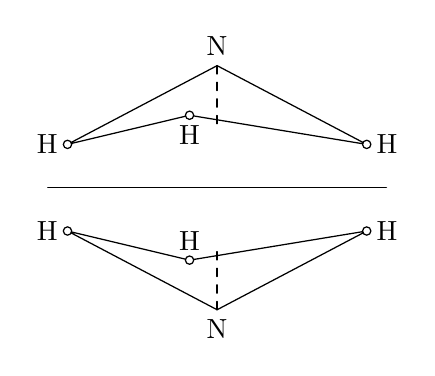
\begin{tikzpicture}[x=1cm,y=1cm,line width=.45pt,line cap=round]
  \draw (-2.15,0)--(2.15,0);
  \coordinate (Lt) at (-1.9,.55); \coordinate (Rt) at (1.9,.55);
  \coordinate (Nt) at (0,1.55); \coordinate (Ct) at (-.35,.92);
  \draw (Lt)--(Nt)--(Rt)--(Ct)--cycle;
  \draw[dashed] (Nt)--(0,.75);
  \filldraw[fill=white] (Lt) circle (1.5pt) (Rt) circle (1.5pt) (Ct) circle (1.5pt);
  \node[left] at (Lt) {H}; \node[right] at (Rt) {H}; \node[above] at (Nt) {N}; \node[below] at (Ct) {H};
  \coordinate (Lb) at (-1.9,-.55); \coordinate (Rb) at (1.9,-.55);
  \coordinate (Nb) at (0,-1.55); \coordinate (Cb) at (-.35,-.92);
  \draw (Lb)--(Nb)--(Rb)--(Cb)--cycle;
  \draw[dashed] (Nb)--(0,-.75);
  \filldraw[fill=white] (Lb) circle (1.5pt) (Rb) circle (1.5pt) (Cb) circle (1.5pt);
  \node[left] at (Lb) {H}; \node[right] at (Rb) {H}; \node[below] at (Nb) {N}; \node[above] at (Cb) {H};
\end{tikzpicture}
\caption{}
\end{figure}

The magnitude of the splitting is proportional to the probability for the atoms to pass through the ``potential barrier'' separating the two molecular configurations. Although this probability is comparatively large in ammonia because of the properties just described, the splitting is nevertheless small ($1\cdot10^{-4}$ eV). An example of a spherical-rotor molecule is treated in Problem 5 of this section.

\subsection*{Problems}

\ProblemHeading 1. Establish the relation between the symmetry of states of the molecule ${}^{12}\mathrm C_2{}^1\mathrm H_4$ and the total spin of its hydrogen nuclei.

\SolutionHeading\footnote{For the method of solving such problems based on permutation-group theory, see the book by I.~G.~Kaplan cited on p.~291, Ch.~VI, \S~2.} The total spin of the four ${}^1\mathrm H$ nuclei can have the values $I=2,1,0$, and its projection $M_I$ ranges from 2 to $-2$. Consider the representations realized by the spin factors belonging to each individual value of $M_I$, beginning with the maximum value.

For $M_I=2$ there is only one spin factor, in which all nuclei have spin projection $+1/2$. For $M_I=1$ there are four different spin factors, distinguished by which of the four nuclei is assigned spin projection $-1/2$. Finally, $M_I=0$ is realized by six spin factors, according to which pair of nuclei is assigned spin projection $-1/2$. The characters of the corresponding three representations are
\[
\begin{array}{c|cccccccc}
 &E&\sigma(xy)&\sigma(xz)&\sigma(yz)&I&C_2(z)&C_2(y)&C_2(x)\\\hline
M_I=2&1&1&1&1&1&1&1&1\\
M_I=1&4&4&0&0&0&0&0&0\\
M_I=0&6&6&2&2&2&2&2&2
\end{array}
\]
The first is the identity representation $A_g$. Since $M_I=2$ can occur only for $I=2$, it follows that spin $I=2$ corresponds to a state of symmetry $A_g$.

The value $M_I=1$ can occur for both $I=1$ and $I=2$. Accordingly subtracting the first representation from the second and decomposing the result into irreducible parts, we find that spin $I=1$ corresponds to the states $B_{1g}$, $B_{2u}$, $B_{3u}$.

Finally, $M_I=0$ can occur in all the cases in which $M_I=1$ is possible, and also for $I=0$. Accordingly subtracting the second representation from the third, we find two states $A_g$ corresponding to spin $I=0$.

\ProblemHeading 2. Determine the symmetry types of the complete (coordinate) wave functions and the statistical weights of the corresponding levels for the molecules

\SourcePage{518}{521}
${}^{12}\mathrm C_2{}^2\mathrm H_4$, ${}^{13}\mathrm C_2{}^1\mathrm H_4$, ${}^{14}\mathrm N_2{}^{16}\mathrm O_4$ (all the molecules have the same shape); the spins are $i({}^2\mathrm H)=1$, $i({}^{13}\mathrm C)=1/2$, $i({}^{14}\mathrm N)=1$.

\SolutionHeading By the same method as was applied in the text to ${}^{12}\mathrm C_2{}^1\mathrm H_4$, we find the following states (the coordinate axes are chosen as in the text):
\[
\begin{array}{c|c|c}
\text{Molecule}&(+)&(-)\\\hline
{}^{12}\mathrm C_2{}^2\mathrm H_4&27A_g,\ 18B_{1g}&18B_{2u},\ 18B_{3u}\\
{}^{13}\mathrm C_2{}^1\mathrm H_4&16A_g,\ 12B_{1g}&12B_{2u},\ 24B_{2u}\\
{}^{14}\mathrm N_2{}^{16}\mathrm O_4&6A_g&3B_{3u}
\end{array}
\]

\ProblemHeading 3. Do the same for the molecule ${}^{14}\mathrm N{}^2\mathrm H_3$.

\SolutionHeading Just as for ${}^{14}\mathrm N{}^1\mathrm H_3$ in the text, we find the states $30A_1$, $3A_2$, $24E$. For the normal electronic and vibrational term, the following states are possible at different values of the quantum number $k$:
\[
\begin{array}{l|cc}&(+)&(-)\\\hline
|k|\text{ not divisible by three}&24E&24E\\
|k|\text{ divisible by three}&30A_1,3A_2&30A_1,3A_2\\
k=0,\ J\text{ even}&30A_1&3A_2\\
k=0,\ J\text{ odd}&3A_2&30A_1
\end{array}
\]

\ProblemHeading 4. Do the same for the molecule ${}^{12}\mathrm C_2{}^1\mathrm H_6$ (see Fig.~43f, symmetry $D_{3d}$).

\SolutionHeading The following types of states are possible: $7A_{1g}$, $1A_{1u}$, $3A_{2g}$, $13A_{2u}$, $9E_g$, $11E_u$.

For the normal electronic and vibrational term, the following states are obtained:
\[
\begin{array}{l|cc}&(+)&(-)\\\hline
|k|\text{ not divisible by three}&9E_g&11E_u\\
|k|\text{ divisible by three}&7A_{1g},3A_{2g}&1A_{1u},13A_{2u}\\
k=0,\ J\text{ even}&7A_{1g}&1A_{1u}\\
k=0,\ J\text{ odd}&3A_{2g}&13A_{2u}
\end{array}
\]

\ProblemHeading 5. Do the same for the methane molecule ${}^{12}\mathrm C{}^1\mathrm H_4$ (the H atoms are at the vertices and the C atom at the center of a tetrahedron).

\SolutionHeading The molecule is a spherical rotor and has symmetry $T_d$. By the same method, we find that states of the following types are possible: $5A_2$, $1E$, $3F_1$ (the corresponding total molecular spins are, respectively, 2, 0, 1). The rotational states of a spherical rotor are classified by the values of the total angular momentum $J$. The $(2J+1)$ rotational functions belonging to a given $J$ realize a $(2J+1)$-dimensional representation of the group $O$, which is isomorphic to $T_d$ and is obtained from it

\SourcePage{519}{522}
by replacing every symmetry plane by a second-order axis perpendicular to it. The characters of this representation are determined by formula (98.3). Thus, for example, for $J=3$ we obtain a representation with characters
\[
\begin{array}{c|ccccc}&E&8C_3&6C_2&6C_4&3C_4^2\\\hline&7&1&-1&-1&-1\end{array}.
\]
It contains the following irreducible representations of $O$: $A_2$, $F_1$, $F_2$. Considering again the rotational structure of the normal electronic and vibrational term, it follows that at $J=3$ states for which the complete wave function has symmetry $A_2$ can only be positive, whereas levels of the state $F_1$ may be either positive or negative. For the first few values of $J$, the following states are obtained in the same way (shown together with their nuclear statistical weights):
\[
\begin{array}{c|cc}&(+)&(-)\\\hline
J=0&-&5A_2\\
J=1&3F_1&-\\
J=2&1E&1E,3F_1\\
J=3&5A_2,3F_1&3F_1\\
J=4&1E,3F_1&5A_2,1E,3F_1
\end{array}
\]
